In this section, we will introduce the partial differential equations posed on parameterized domains.
First, we will introduce the Poisson problem, which will be followed by the Helmholtz scattering problem.

\subsection{Poisson equation}\label{subsec:poisson-shape}
We consider the elliptic diffusion equation on a family of open Lipschitz domains ${D}(\y)\subset \mathbb{R}^2$, parameterized by $\y\in Y$:
\begin{equation}
    \begin{cases}
        -\nabla\cdot \left(a\nabla \uparamdomain(\y) \right) = f, & \text{in } {D}(\y),\\
        \uparamdomain(\y) = 0, & \text{on } \partial {D}(\y),\\
        \text{for every  }\bm{y} \in Y,
    \end{cases} \label{eq:shapepoisson}
\end{equation}
where $a\in L^\infty(\mathcal{D}_H), f\in L^2(\mathcal{D}_H)$ are analytic functions from the hold-all domain $\mathcal{D}_H = \cup_{\y\in Y}{D}(\y)$ to $\mathbb{R}$, fixed and independent of $\y\in Y$.
We distinguish $\uparamdomain$, the solution on the parameterized domain, from $u$, which will later be the solution on a fixed domain.
Finally, we assume that $a$ and $f$ satisfy the following regularity assumption:
\begin{assumption}\label{ass:analytic}
Both $a$ and $f$ in~\eqref{eq:shapepoisson} are analytic functions from $\mathcal{D}_H$ to $\mathbb{R}$.
Next to this, we have that the coefficient $a$ is uniformly bounded by
\begin{equation*}
    0 < a_{\min} \leq a(\x) \leq a_{\max} < \infty,
\end{equation*}
for some constants $a_{\min},a_{\max}>0$.
\end{assumption}
For each $\y \, \in \, Y$, the variational formulation of~\eqref{eq:shapepoisson} reads:
\begin{align}
    &\text{find }\uparamdomain(\y) \in V\coloneqq H_0^1(\Dy)  \text{ such that}\nonumber \\
    &\qquad\int_{\Dy} a \nabla \uparamdomain(\y) \cdot \nabla v \d \bm{x} = \int_{\Dy} f v\d \bm{x}, \quad \text{ for all } {v} \in V. \label{eq:variational_formulation_y_poission}
\end{align}
Thanks to the assumptions on $a$ and $f$, the Lax-Milgram lemma ensures well-posedness for every $\y \in Y$.

We will consider parameterized star-shaped domains in $\mathbb{R}^2$ such that we can efficiently define the domain parameterization in Section~\ref{subsec:expansion-basis}.
Moreover, this star shaped property opens the door to an explicit treatment of the domain parameterization which we will discuss in Section~\ref{subsubsec:mapping-approach}.
To ensure the star-shape property, we express the parameterized domains ${D}(\y)$ in polar coordinates as the region inside a simple, closed curve $r_0(\y,\theta)$ with $\theta\in[0,2\pi)$ and $\y\in Y$:
\begin{equation}
    {D}(\y) = \{ \x \in \mathbb{R}^2: |\x| \leq r(\y,\theta(\x)) \},\label{eq:starshapepossiondomain}
\end{equation}
where $r \in C^{0, 1}_{per}([0, 2\pi))$ parameterizes the boundary of the domain ${D}(\y)$ in terms of the parameter $\y$ and where $\theta(\x)$ denotes the argument of $\x\in\mathbb{R}^2$.
Figure~\ref{fig:poissonsketch} provides a sketch of the outlined situation.


\subsection{Helmholtz equation}\label{subsec:helmholtz-shape}
For the Helmholtz equation, we consider an exterior scattering problem where an incoming wave $u_{in}$ scatters against a star-shaped object centered at the origin.
This scatter is assumed to be from a family of open Lipschitz domains ${D}(\y)\subset \mathbb{R}^2$ as well, and we will consider sound-soft scattering at the boundary of the scatterer.
The resulting variational formulation is:
Find $\mathrm{u}(\y) \in V\coloneqq H^1_{0, \Gamma_{scat}}({D}(\y))$ such that:
\begin{align}
    \int_{{D}(\y)} a_{out}\nabla \uparamdomain(\y) \cdot \nabla v \dx &-k^2\int_{{D}(\y)} n_{out}  \uparamdomain(\y) v \dx -ik\int_{\Gamma_{out}} \uparamdomain(\y) v \dx \nonumber\\
    &= \int_{\Gamma_{out}} \left( \frac{\partial}{\partial\bm{n}} -ik\right) u_{in} v \dx,\label{eq:varformhelmholtz_shape}
\end{align}
for all $\y \in Y$ and all $v\in V$, where $a_{out}$ and $n_{out}$ are defined on the hold-all domain $\mathcal{D}_H=\cup_{\y\in Y}{D}(\y)$ satisfying~\cite[Assumption~2.4]{graham2019} such that they define a nontrapping problem~\cite[Theorem~2.5]{graham2019}\footnote{To use this result, we require the boundary excitation to be zero. This is not true for our total field equations, but we can use a bound on the linear combination of the scattered field and the total field, such as in~\cite[Corollary~1.6]{chaumont-frelet2023} to obtain the required results.}.
In our case, we take $a_{out}$ and $n_{out}$ constant, both spatially and parametrically, and set them to one such that, together with the star-shaped property of $D_{scat}(\y)$, we satisfy Assumption~\ref{ass:nontrapping}~\cite[Prop. 3.1, Chapter 5]{lax1989} with the constant $C_{\text{bound}}$ independent of $\y$~\cite{chandler-wilde2008}.
Again, we distinguish $\uparamdomain$, the solution on the parameterized domain, from $u$, which will later be the solution on a fixed domain.

Similar to the Poisson example, we assume that the central scatterer is parameterized by $\y\in Y$:
\begin{equation}
    D_{scat}(\y) = \{ \x \in \mathbb{R}^2: |\x| \leq r(\y,\theta(\x)) \},\label{eq:starshapescat}
\end{equation}
where $r \in C^{0, 1}_{per}([0, 2\pi))$ parameterizes the boundary $\Gamma_{in}$ of the domain $D_{scat}(\y)$ in terms of the parameter $\y$ and where $\theta(\x)$ denotes the argument of $\x\in\mathbb{R}^2$.
To truncate the domain, we introduce a circular outer boundary $\Gamma_{out}$ with radius $r_{out}$ such that $\esssup_{\theta, \y} r(\y,\theta) < r_{out}$, ensuring that $\Gamma_{out}$ completely encompasses the central scatterer $D_{scat}(\y)$ for all $\y \in Y$.
Therefore, the computational domain becomes
\begin{equation*}
    {D}(\y) = \{ \x \in \mathbb{R}^2:  r(\y,\theta(\x)) \leq |\x| \leq  r_{out}\},\label{eq:starshapehelmholtzdomain}
\end{equation*}
which is sketched schematically in Figure~\ref{fig:helmholtzsketch}.

\begin{figure}
    \centering
    \begin{subfigure}[b]{0.49\textwidth}
        \centering
        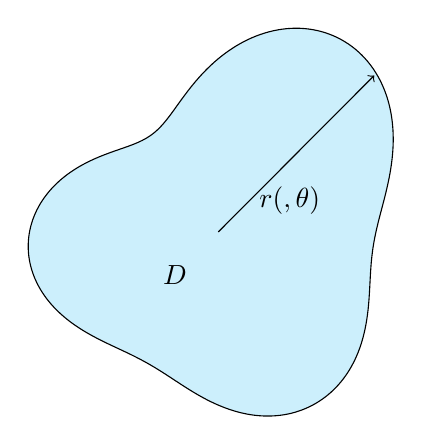
\begin{tikzpicture}[scale=2.2]
            \draw[fill=cyan!20,domain=0:3*pi,samples=500,fill opacity=1,shift={(-2,0)}] plot ({deg(\x)}:{((0.6*cos(\x * 1 r)^3 - 1.05*cos(\x * 3 r) + sin(\x*2 r)*0.5)*0.2+1)});
            \node at (-2.25,-0.25) {$D$};
            \draw[->,shift={(-2,0)}] (0,0) -- (0.9, 0.903) node [pos=0.2, right] {$r(\y, \theta)$};
        \end{tikzpicture}
        \caption{}\label{fig:poissonsketch}
    \end{subfigure}%
    ~
    \begin{subfigure}[b]{0.49\textwidth}
        \centering
        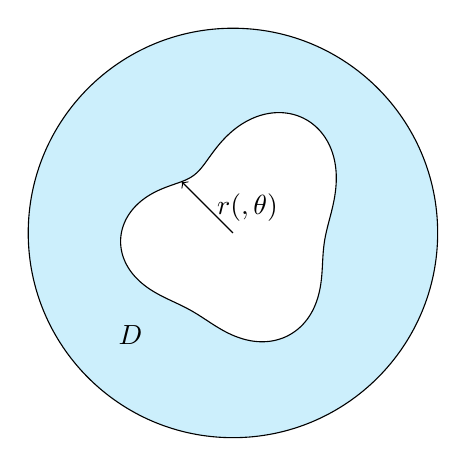
\begin{tikzpicture}[scale=1.3]

            % Annular region: draw filled between circle and perturbed circle
            \begin{scope}
                % Outer circle path (radius 1)
                \draw[fill=cyan!20, opacity=1, even odd rule, shift={(-2,0)}]
                (0,0) circle(2)
                % Inner perturbed path (reverse direction for -even odd rule-)
                [shift={(0,0)}]
                plot[smooth, domain=0:360, samples=400]
                ({(((0.6*cos(\x)^3 - 1.05*cos(\x * 3) + sin(\x*2)*0.5)*0.2+1) * cos(\x)},
                    {((0.6*cos(\x)^3 - 1.05*cos(\x * 3) + sin(\x*2)*0.5)*0.2+1) * sin(\x)});
            \end{scope}
            \node at (-3,-1) {$D$};

            \draw[->,shift={(-2,0)}] (0,0) -- (-0.5, 0.5) node [pos=0.5, right] {$r(\y, \theta)$};
        \end{tikzpicture}
        \caption{}\label{fig:helmholtzsketch}
    \end{subfigure}
    \caption{Schematic sketches of the parameterized domains in both the Poisson problem (a) and the exterior Helmholtz scattering problem (b).}
\end{figure}